\documentclass[11pt]{article}
\usepackage{fullpage,amsmath,mathtools, algorithm2e, forest}
\usepackage[mathletters]{ucs}
\usepackage{hyperref}
\usepackage[utf8x]{inputenc}
\usepackage{graphicx}
\usepackage{listings}
\usepackage{courier}

\lstset{basicstyle=\footnotesize\ttfamily,breaklines=true}
\lstset{frame=single}

\graphicspath{ {./images/} }
\title{COMP4107 - Assignment 2}
\author{Student Name: Yunkai Wang\\
\text{Student Number: 100968473}\\\\
Student Name: Jules Kuehn\\
\text{Student Number: 100661464}}
\date{Fall 2018}
\begin{document}
\maketitle
\begin{enumerate}

\item
a) The graphs and tables below can be reproduced by running the relevant q1*.py file.\newline
\newline
The 10x10 grid described in the assignment was created and the order randomized. The actual values z = f(x,y) were computed and stored in a matrix representing [x, y, z] for all 100 training items. After training on the 10x10 grid for 50,000 epochs, error predicting z values from the test data (the 9x9 grid) was very low for both 8 neurons and 50 neurons. Note that using 2 neurons shows to be insufficient to approximate the function in both dimensions.\newline
\begin{figure}[h!]
    \centering
    \begin{minipage}{0.45\textwidth}
        \centering
        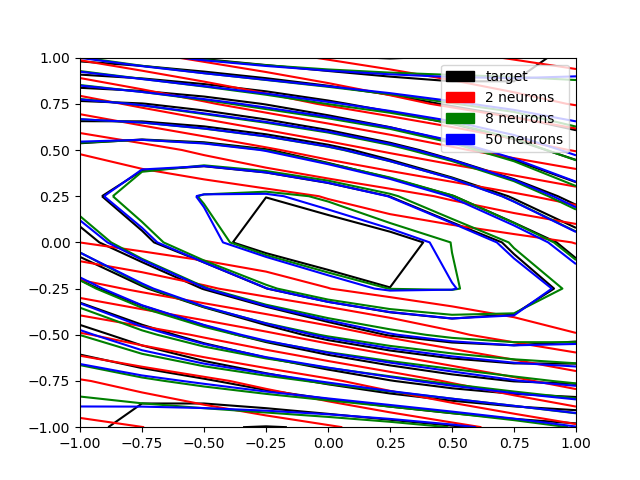
\includegraphics[width=0.9\textwidth]{q1a-2} % first figure itself
        \caption{Function Contours}
    \end{minipage}\hfill
    \begin{minipage}{0.45\textwidth}
        \centering
        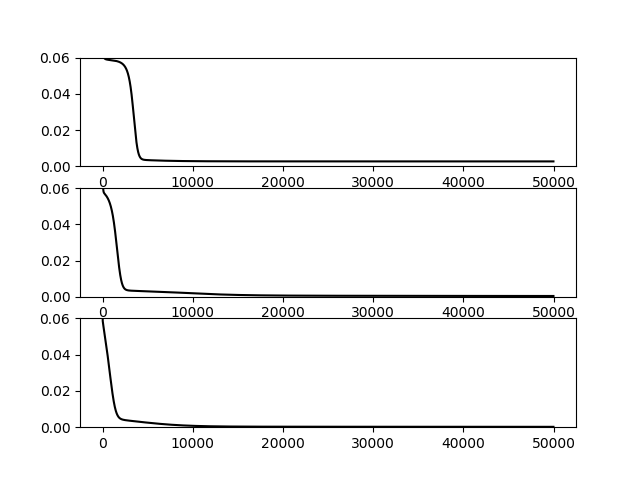
\includegraphics[width=0.9\textwidth]{q1a-2-costs} % second figure itself
        \caption{Cost (MSE) at epoch}
    \end{minipage}
\end{figure}\newline
Using 8 neurons for the hidden layer is appropriate for this function. The MSE for the test data with 8 neurons is better that is required, and the training converges after fewer epochs than the network using 50 neurons for the hidden layer.\newline
\newline
The table below corresponds to the experiment shown in the graph above.\newline
\lstinputlisting{python_output/q1a-results.txt}


b) With a tolerance of 0.02 for MSE of the training data, the appropriate number of epochs for convergence varies by training method. For traingrms (RMSPropOptimizer), having a maximum of 100 training epochs is appropriate. The other methods converge much more slowly, as seen in Figure 3. \newline

\begin{figure}[h!]
    \centering
    \begin{minipage}{0.45\textwidth}
        \centering
        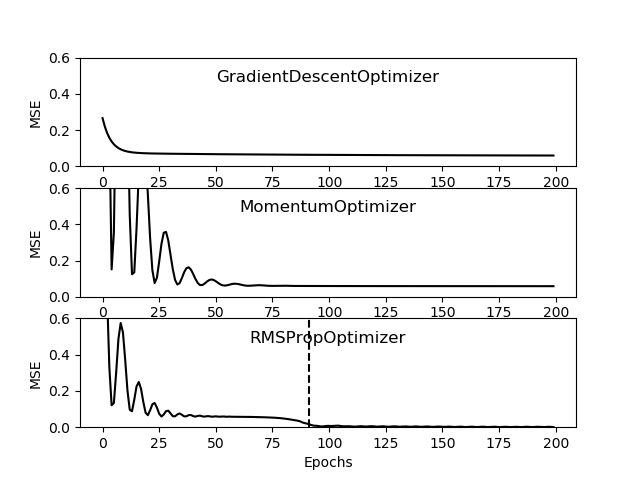
\includegraphics[width=0.9\textwidth]{q1b-2b} % first figure itself
        \caption{Convergence vs optimizer}
    \end{minipage}\hfill
    \begin{minipage}{0.45\textwidth}
        \centering
        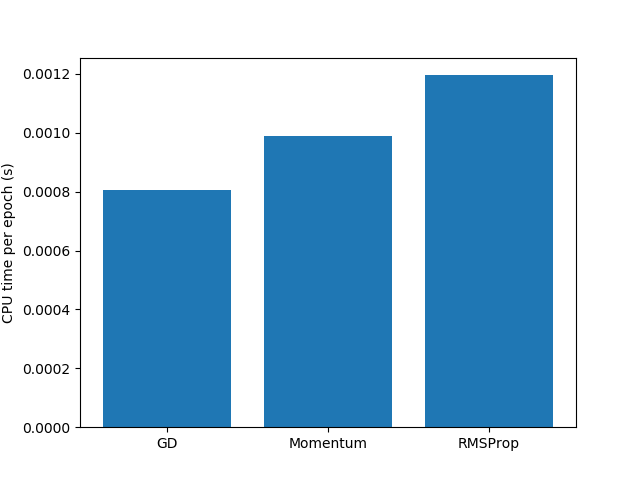
\includegraphics[width=0.9\textwidth]{q1b-3_cpu-time} % second figure itself
        \caption{CPU time vs optimizer}
    \end{minipage}
\end{figure}

The reduced number of required training epochs for RMSPropOptimizer (seen in the table below) more than compensates for the increased CPU time for each epoch, seen in Figure 4.\newline
\lstinputlisting{python_output/q1b-results.txt}


c) We can further show that 8 neurons is a good choice by noting that early stopping has no effect. Our experiments have not been able to demonstrate an overtraining phenomenon with even 50 hidden neurons, but a premature early stop can be seen in Figure 6, and the table below.\newline
\lstinputlisting{python_output/q1c-results.txt}

\begin{figure}[h!]
    \centering
    \begin{minipage}{0.45\textwidth}
        \centering
        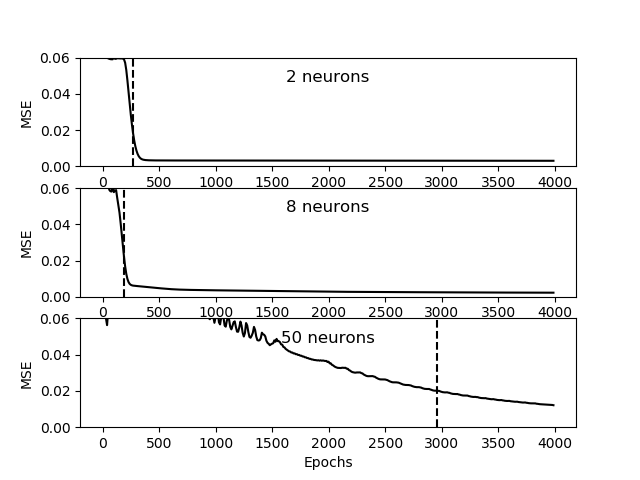
\includegraphics[width=0.9\textwidth]{q1c-1-50_neurons_slow_convergence2} % first figure itself
        \caption{Slow convergence}
    \end{minipage}\hfill
    \begin{minipage}{0.45\textwidth}
        \centering
        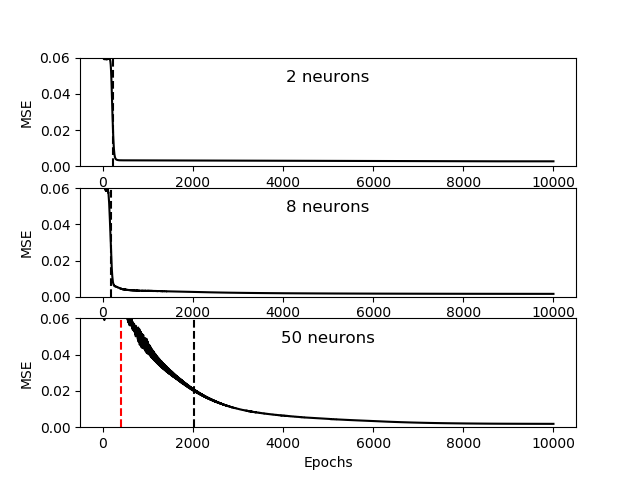
\includegraphics[width=0.9\textwidth]{q1c-2-earlyStopping} % second figure itself
        \caption{Premature early stop}
    \end{minipage}
\end{figure}

The network with 50 hidden neurons also is very slow to converge to the target MSE - even using the RMSPropOptimizer - compared to when using 8 hidden neurons (Figure 5).\newline

\begin{figure}[h!]
    \centering
    \begin{minipage}{0.45\textwidth}
        \centering
        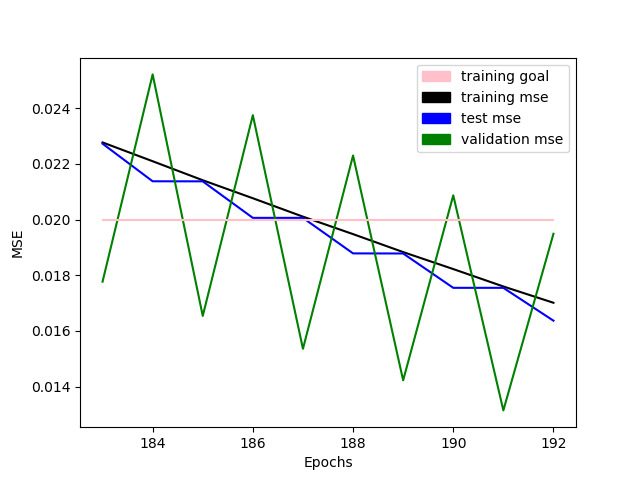
\includegraphics[width=0.9\textwidth]{q1c-3} % first figure itself
        \caption{Reaching training goal}
    \end{minipage}\hfill
    \begin{minipage}{0.45\textwidth}
        \centering
        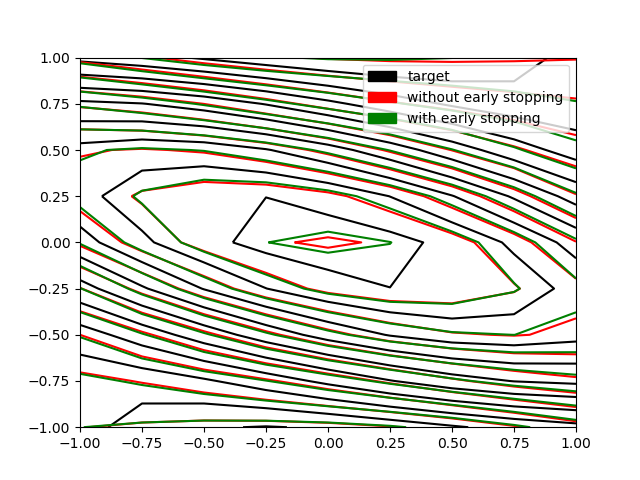
\includegraphics[width=0.9\textwidth]{q1c-32} % second figure itself
        \caption{Early stopping not triggered}
    \end{minipage}
\end{figure}

Figure 7 shows the MSE at each epoch near where the training goal is reached. This captures the expected trend - that the training error will decrease consistently, while the test error (9x9 grid) has more variation. The validation data is most different from the training data (as it is randomly sampled from the function), so it is expected that its error would also have the highest variance.\newline
\newline
Figure 8 shows that having an early stopping mechanism for this function makes no difference, as the early stopping mechanism is never triggered (8 hidden neurons, 4000 epochs, 0.02 LR). Thus, the two contours are virtually identical, differing only by the stochastic elements of the experiments (initial weights, order of training data). 


\item Instructions on how to run q2.py:\newline
\newline
Running q2.py without changing anything will run all three parts. This may take a while as it runs 10 experiments for each number of hidden neurons, and after one is finished, a new NN is created to run the second one, etc. Therefore, it will take about 1 min for it to finish and plot the graphs. If you want to run parts only, then comment out the corresponding line in the experiment function.\\
We started by using the default learning rate for AdamOptimizer (0.001). This took 400-700 epochs to converge to the result. However, if we use 0.01 as the learning rate, it converges faster -- within 100 epochs every time. Therefore, we chose 0.01 as the learning rate for this question.\\

% \lstinputlisting{python_output/q2.out}
% 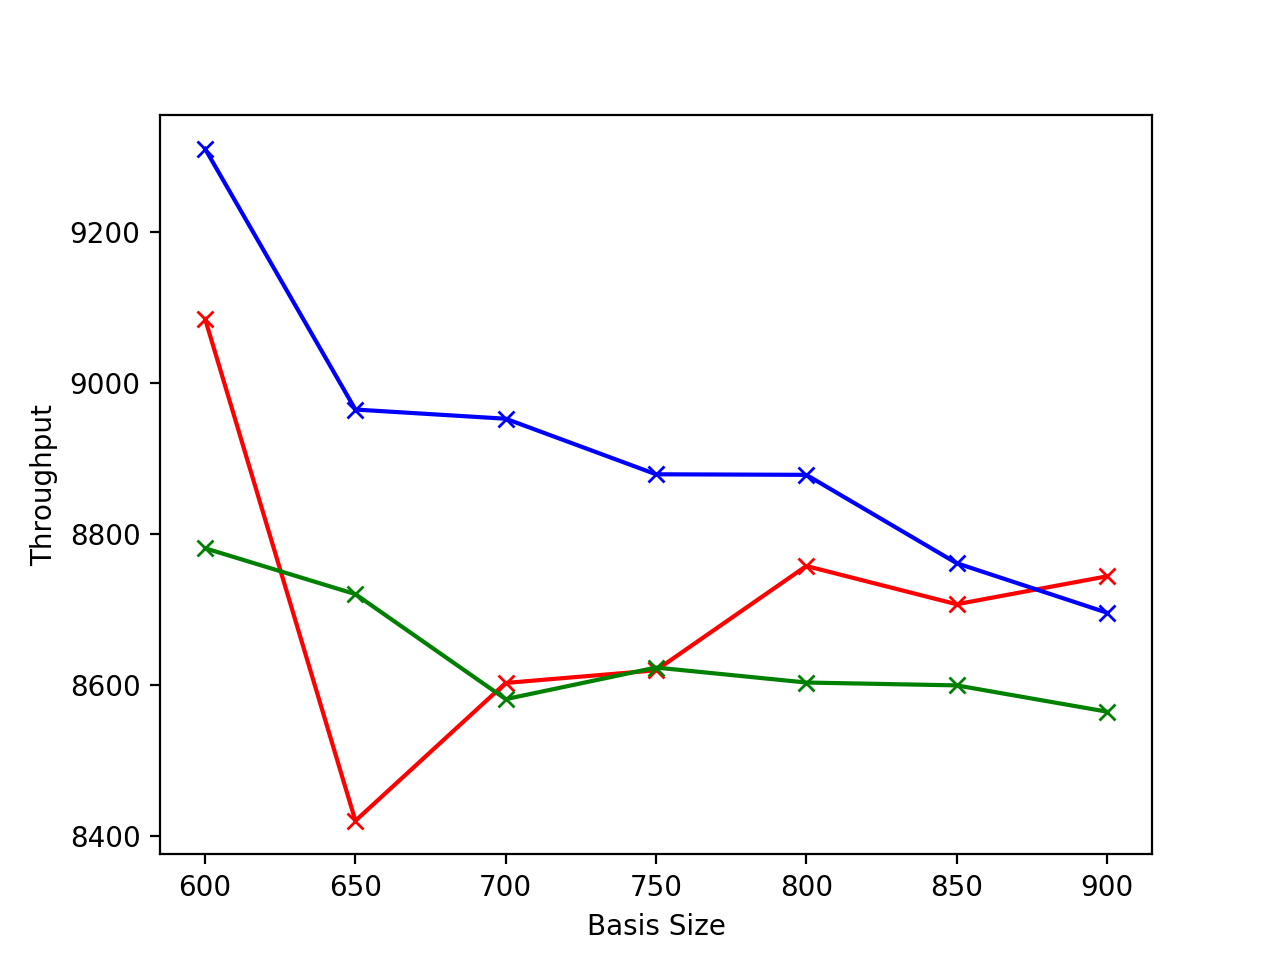
\includegraphics[width=0.7\columnwidth]{q7_result3}
\begin{enumerate}
\item We took the averages of 10 experiments for each of 5, 10, 15, 20, and 25 hidden neurons. These are plotted with red (5), blue (10), green (15), black (20), and purple (25) lines.\newline

\begin{figure}[h!]
    \centering
     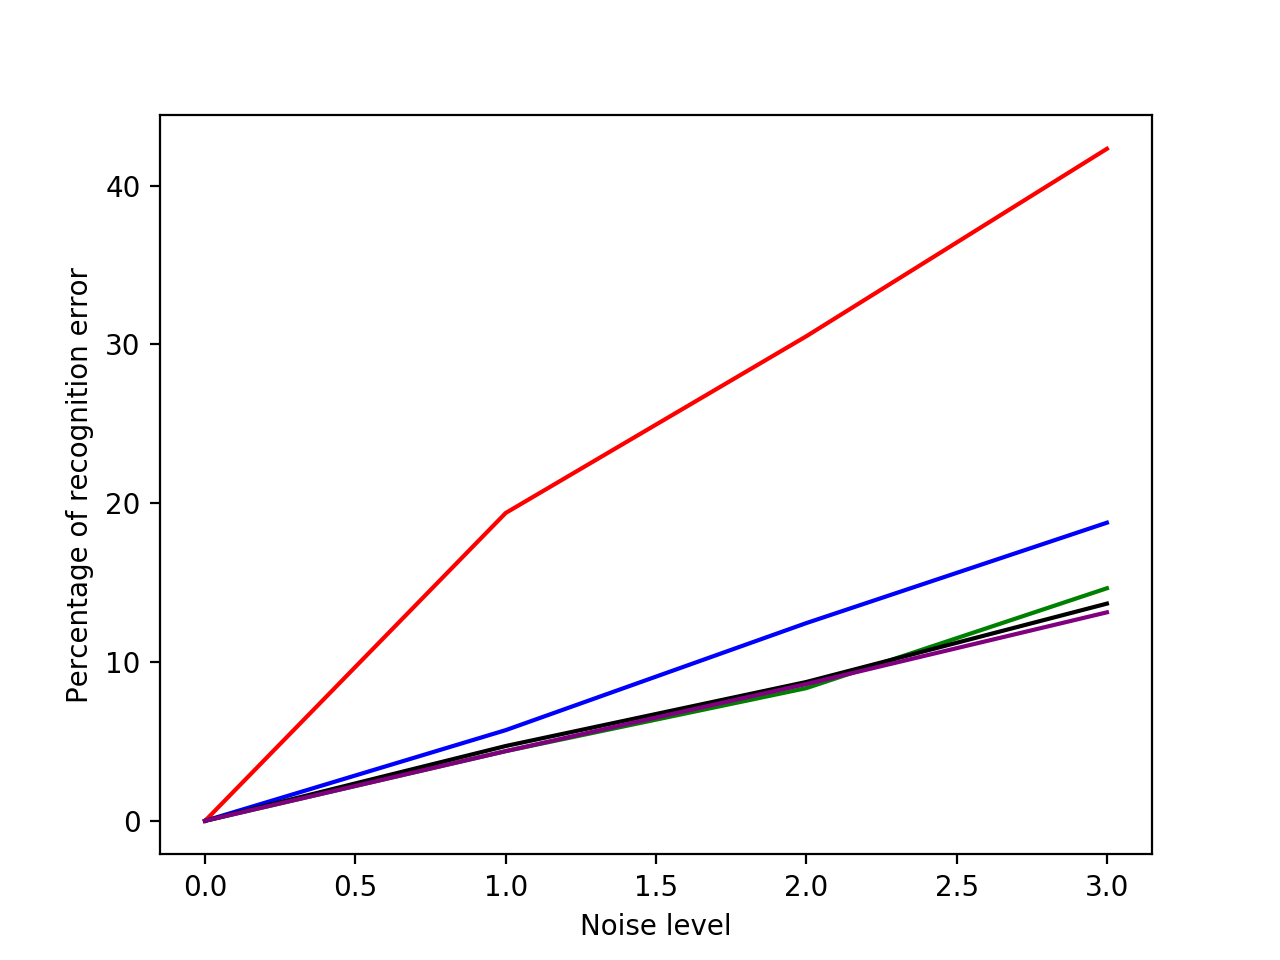
\includegraphics[height=0.5\textwidth, width=0.5\textwidth]{q2-a-1}
        \caption{Percentage of Recognition Errors}
\end{figure}
\begin{figure}[h!]
    \centering
     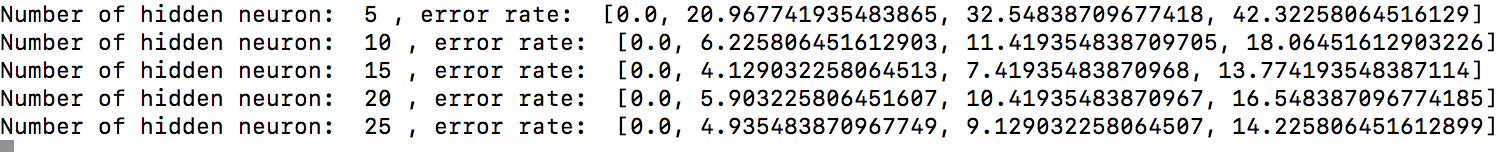
\includegraphics[width=0.9\textwidth]{q2-a-accuracy}
        \caption{Error rate for different number of hidden neurons}
\end{figure}

\item 15 is chosen as the number of hidden neurons, since 15 is more accurate than 10, but using more than 15 neurons is less accurate on the noisy data. When we used 15 neurons in the hidden layer, the number of epochs to reach zero errors is much less than is shown in the assignment question, which we think is fine. Perhaps this is due to a different learning rate.\\
\begin{figure}[h!]
    \centering
    \begin{minipage}{0.45\textwidth}
    	\centering
        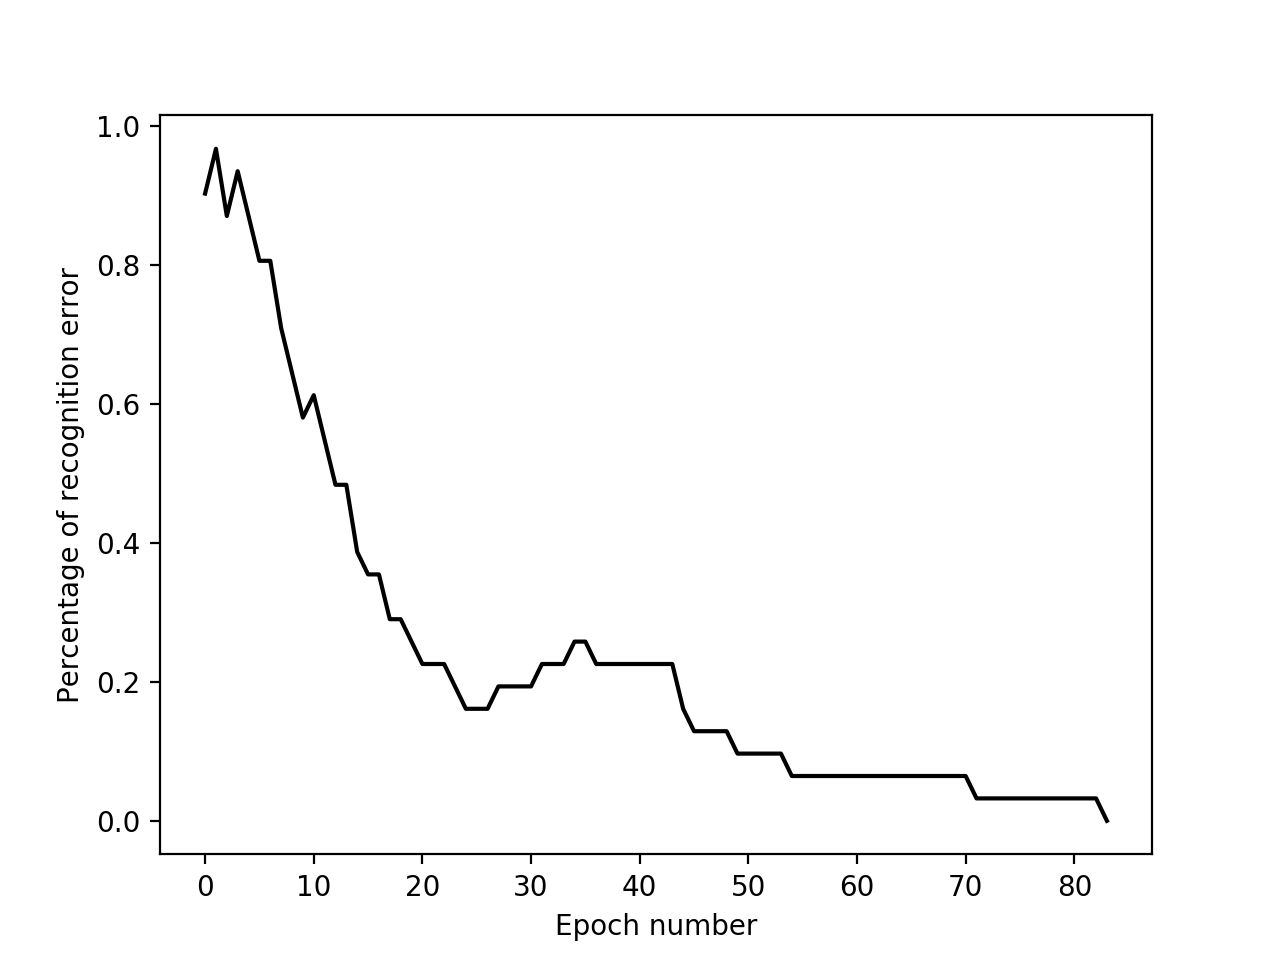
\includegraphics[width=0.9\textwidth]{q2-b-1} % first figure itself
        \caption{Training on perfect data}
    \end{minipage}\hfill
    \begin{minipage}{0.45\textwidth}
    	\centering
         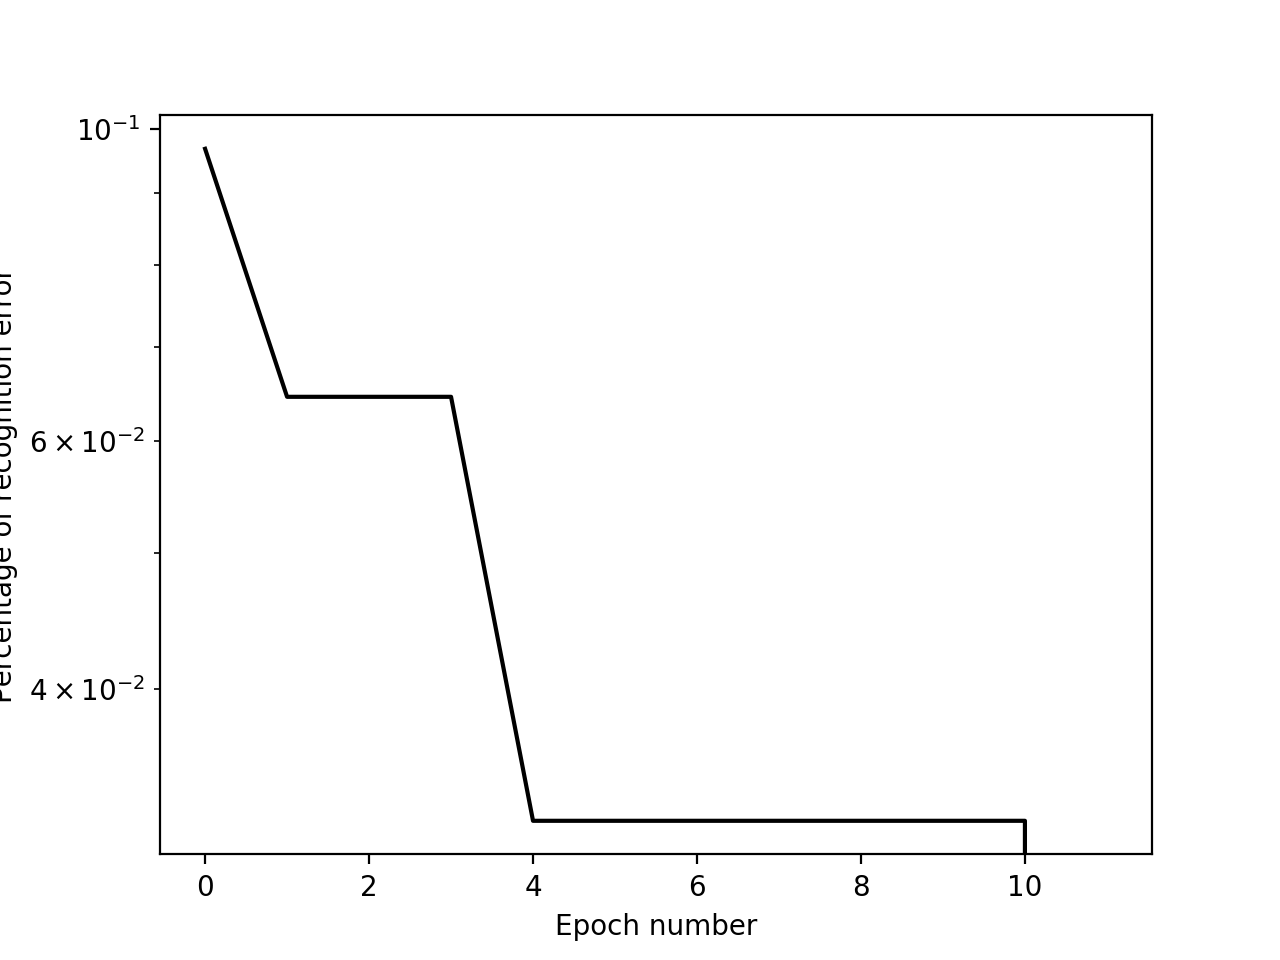
\includegraphics[width=0.9\textwidth]{q2-b-2} % first figure itself
         \caption{Re-training after noisy data}
    \end{minipage}\hfill
\end{figure}

\item The network trained with both perfect and noisy data performed just as well on perfect data, and better on noisy data. The chart below is for the network with 15 neurons. The blue dashed line is trained with only perfect data, and the red line is trained with both perfect and noisy data.\\
\begin{figure}[h!]
    \centering
     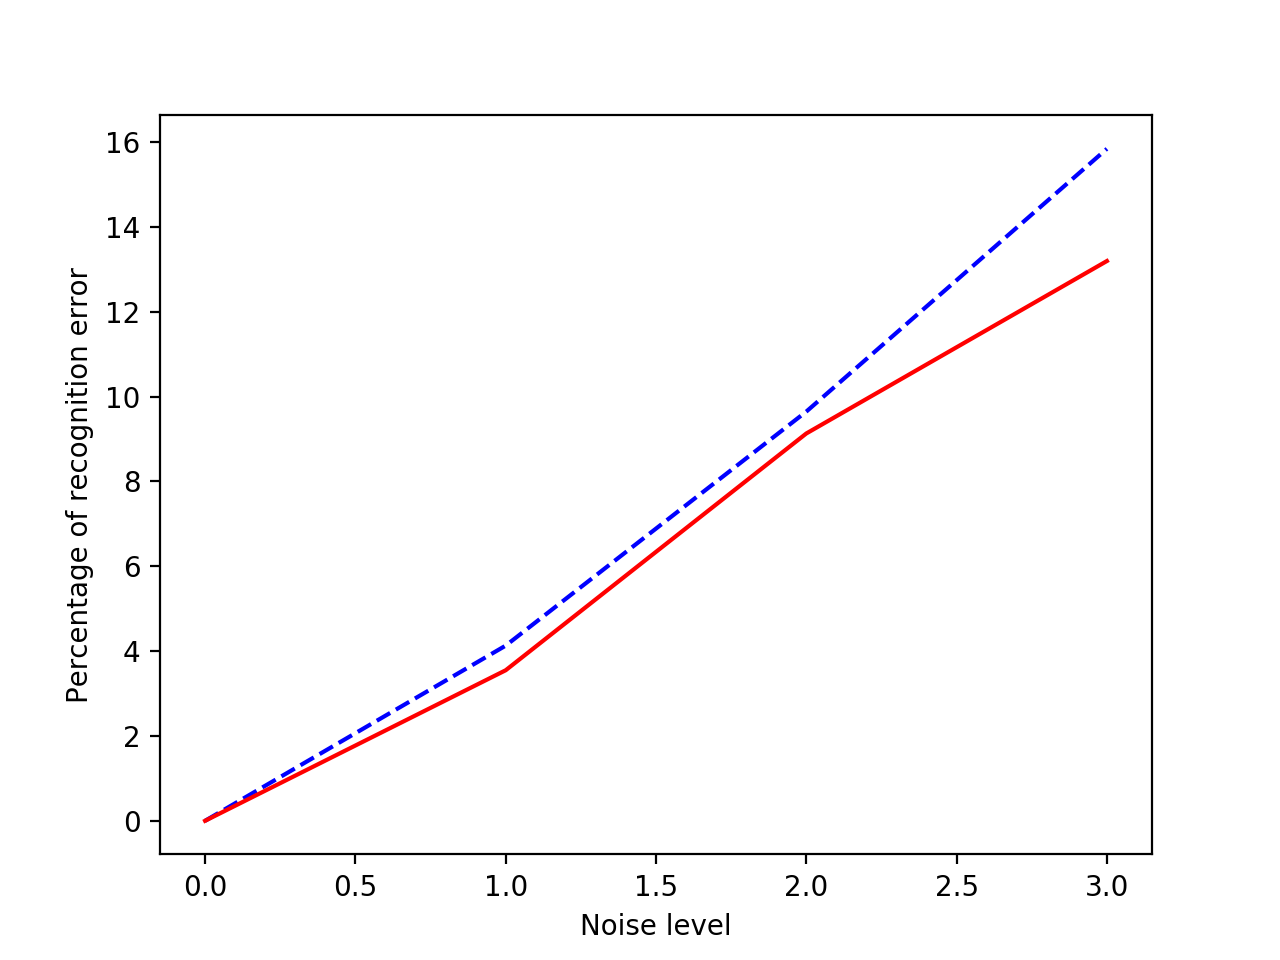
\includegraphics[height=0.5\textwidth, width=0.5\textwidth]{q2-c}
        \caption{Percentage of Recognition Errors}
\end{figure}

\end{enumerate}

\end{enumerate}
\end{document}